66. $\cfrac{(x^2-4x-1)(x^2-8x+16)}{(x^2+x)(x^2-16x+64)}\geqslant0\Leftrightarrow
\cfrac{(x-(2-\sqrt{5}))(x-(2+\sqrt{5}))(x-4)^2}{x(x+1)(x-8)^2}\geqslant0.$ Применив метод интервалов, найдём ответ: $x\in
(-\infty;-1)\cup[2-\sqrt{5};0)\cup\{4\}\cup[2+\sqrt{5};8)\cup(8;+\infty).$
\begin{figure}[ht!]
\center{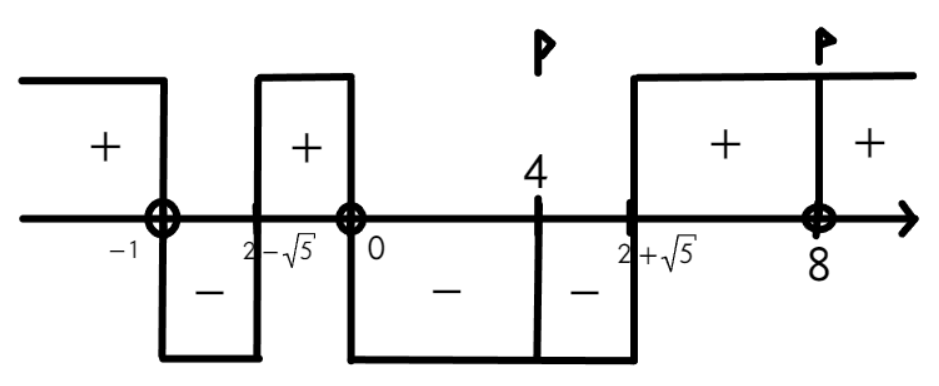
\includegraphics[scale=0.35]{ner9-66.png}}
\end{figure}\\
